\section{Results}
\subsection{PoseNet}
Several pretrained models can be used as features extractor in the PoseNet structure. In \cref{tab:mapnet-backends} are presented the most powerful ones for features extraction tested on the same final linear encoder. The overall trend is similar, this highlights that the extracted features are enough for the task independently of the backbone used.
\begin{table}[htbp]
    \caption{PoseNet backend comparison}
    \begin{center}
        \begin{tabular}{lrrrr}
            \toprule
            {Model}         & \thead{Position                                        \\error} & \thead{Rotation\\error} & \thead{Total\\parameters} & \thead{Trainable\\parameters} \\
            \midrule
            GoogLeNet       & 0.781           & 0.119          & -          & -      \\
            ResNet-18       & 0.635           & 0.288          & 11,180,103 & 3,591  \\
            ResNet-34       & 0.632           & 0.223          & 21,288,263 & 3,591  \\
            ResNet-50       & 0.707           & 0.191          & 23,522,375 & 14,343 \\
            ResNet-152      & \textbf{0.594}  & \textbf{0.139} & 58,158,151 & 14,343 \\
            EfficientNet-B7 & 0.817           & 0.132          & 63,804,887 & 17,927 \\
            \bottomrule
        \end{tabular}
        \label{tab:posenet-backends}
    \end{center}
\end{table}

\begin{table}[htbp]
    \caption{PoseNet losses comparison}
    \begin{center}
        \begin{tabular}{lrr}
            \toprule
            Loss             & {Position Error} & {Rotation Error} \\
            \midrule
            SmoothedL1Loss   & \textbf{0.594}  & \textbf{0.139} \\
            L1Loss           & 0.906           & 0.226          \\
            MSE              & NaN             & NaN            \\
            weighted\_custom & NaN             & NaN            \\
            \bottomrule
        \end{tabular}
        \label{tab:posenet-backends}
    \end{center}
\end{table}

\begin{figure}[h]
    \begin{center}
        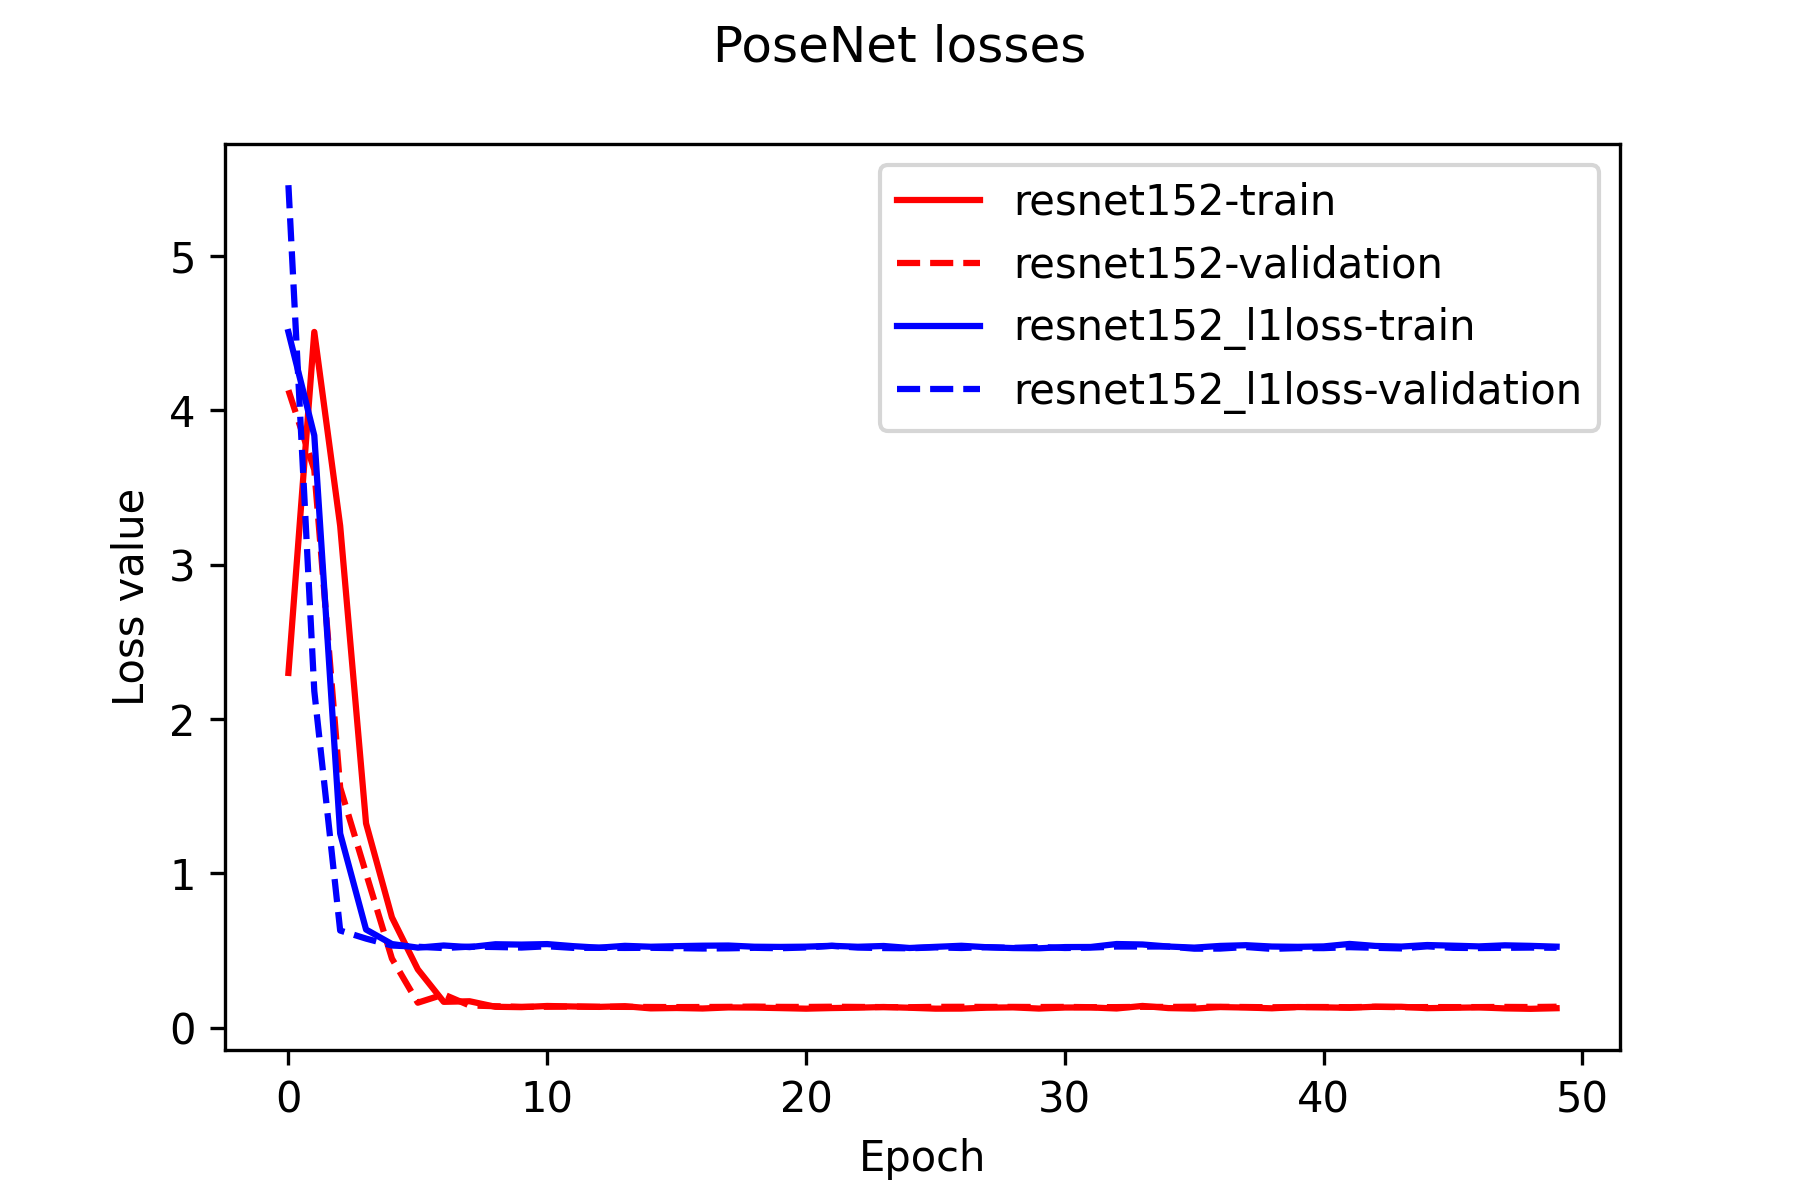
\includegraphics[width=0.50\textwidth]{./imgs/posenet_losses.png}
    \end{center}
    \caption{PoseNet (ResNet-152) losses}
    \label{fig:posenet-losses}
\end{figure}

\begin{figure*}[h]
    \begin{center}
        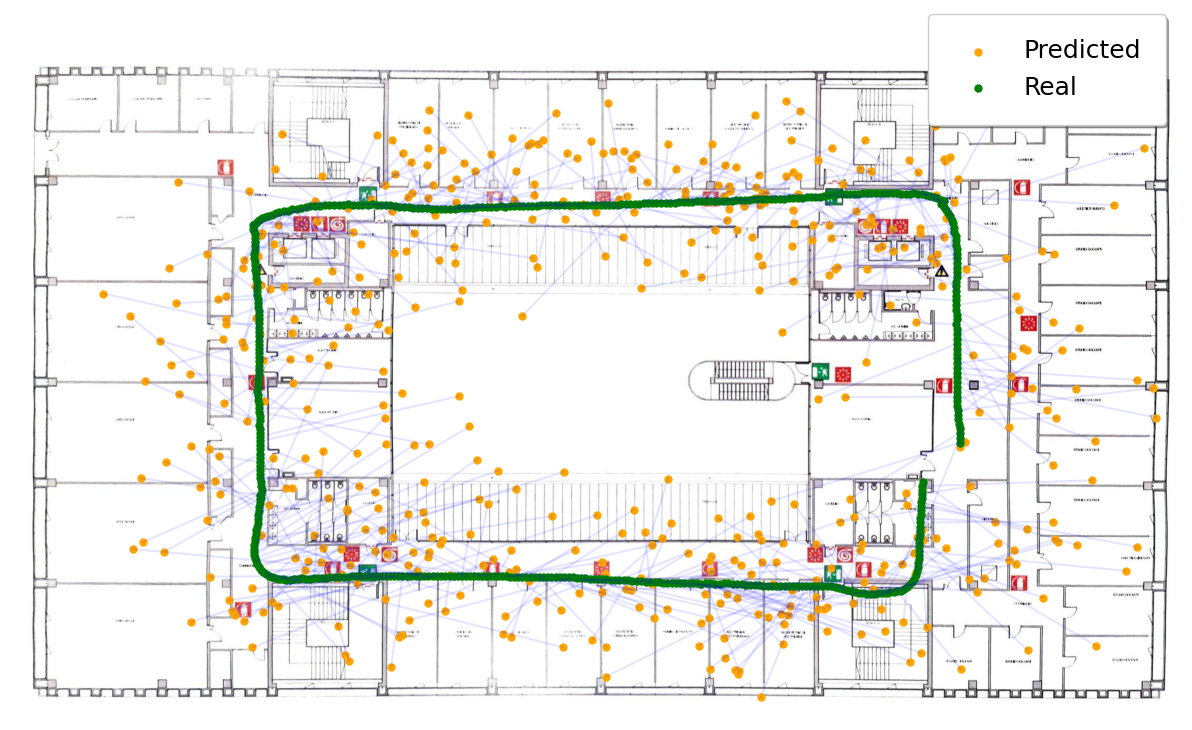
\includegraphics[width=0.95\textwidth]{./imgs/posenet_map.png}
    \end{center}
    \caption{Predicted trajectory PoseNet}
    \label{fig:trajectory-posenet}
\end{figure*}


\subsection{MapNet}
Several pretrained models can be used as features extractor in the MapNet structure. In \cref{tab:mapnet-backends} are presented the most powerful ones for features extraction tested on the same final linear encoder. The overall trend is similar, this highlights that the extracted features are enough for the task independently of the backbone used.
\begin{table}[htbp]
    \caption{MapNet backend comparison}
    \begin{center}
        \begin{tabular}{lrrrr}
            \toprule
            {Model}         & \thead{Position                                            \\error} & \thead{Rotation\\error} & \thead{Total\\parameters} & \thead{Trainable\\parameters} \\
            \midrule
            GoogLeNet       & 0.225           & 0.0876          & -          & -         \\
            ResNet-18       & 0.202           & 0.0658          & 14,853,703 & 3,677,191 \\
            ResNet-34       & \textbf{0.187}  & \textbf{0.0757} & 24,961,863 & 3,677,191 \\
            ResNet-50       & 0.220           & 0.0969          & 30,330,951 & 6,822,919 \\
            ResNet-152      & 0.233           & 0.0869          & 64,966,727 & 3,677,191 \\
            EfficientNet-B7 & 0.210           & 0.0848          & 71,658,455 & 7,871,495 \\
            \bottomrule
        \end{tabular}
        \label{tab:mapnet-backends}
    \end{center}
\end{table}

Another point that emerges is the importance of the final encoder, it works similarly of the \textit{bag of words} used by structure from motion (link al paper). Extracted features are mapped in a space that is used later as a comparison tool for new images for which the pose is asked.
For this reason the final encoder was modified from the original one (link al paper) in order to increase the latent space in which data can be stored.

\begin{figure*}[h]
    \begin{center}
        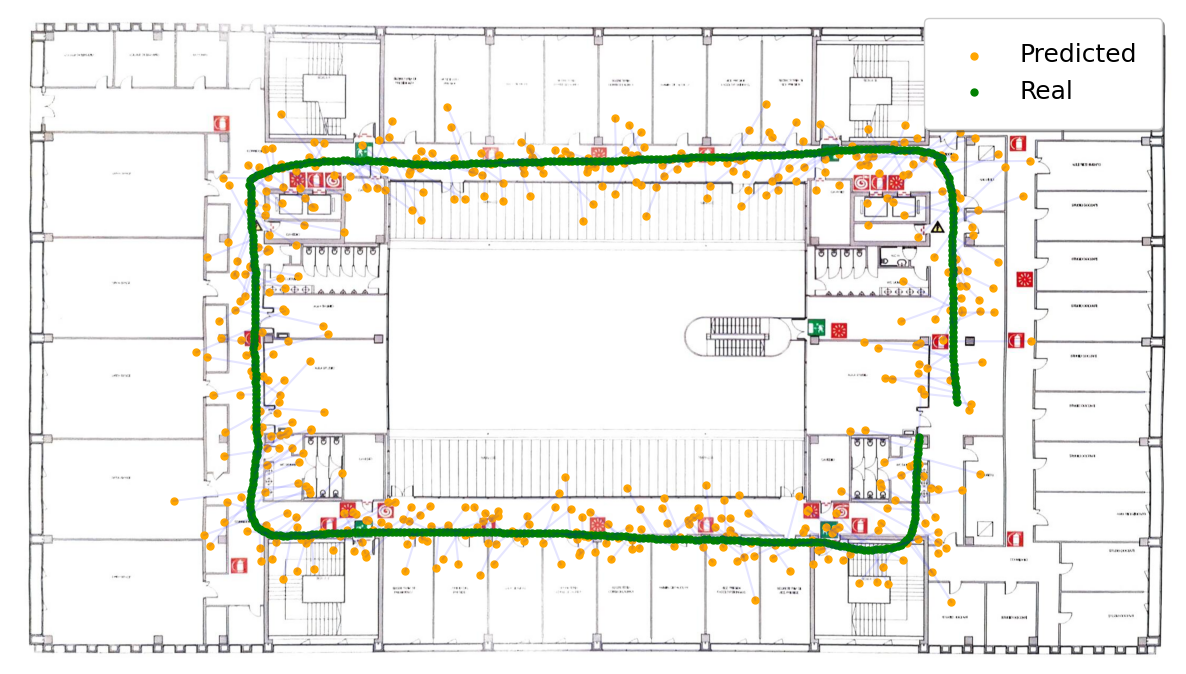
\includegraphics[width=0.95\textwidth]{./imgs/mapnet_map.png}
    \end{center}
    \caption{Predicted trajectory MapNet}
    \label{fig:trajectory-mapnet}
\end{figure*}

\subsection{Comparison}
\begin{figure*}[h]
    \begin{center}
        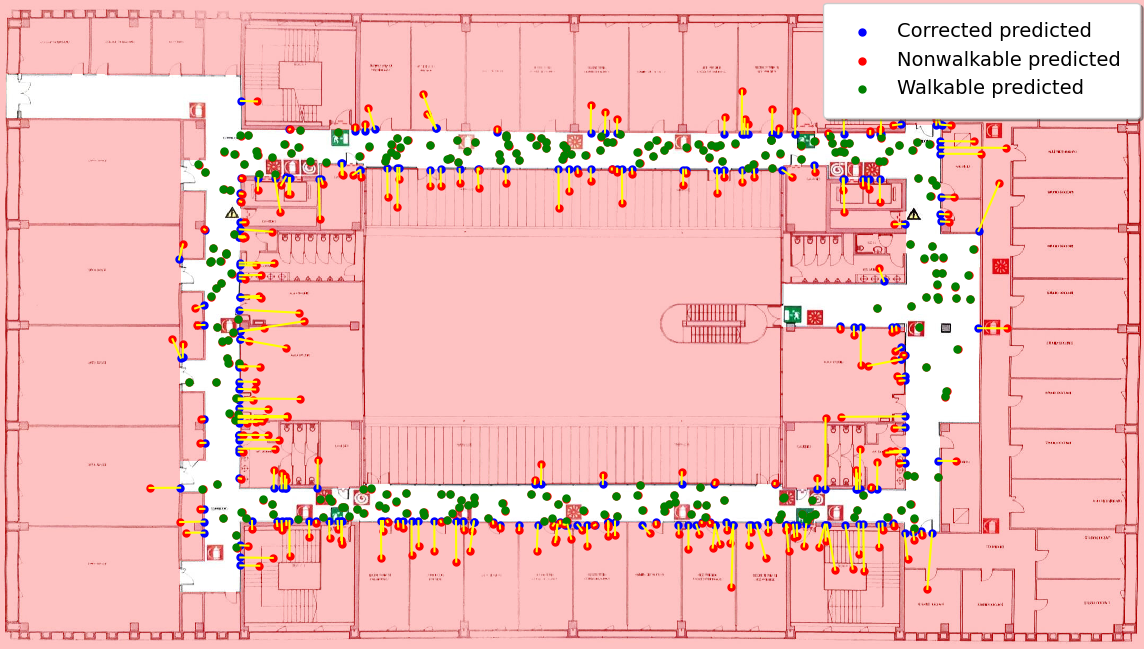
\includegraphics[width=0.95\textwidth]{./imgs/walkable_postprocess.png}
    \end{center}
    \caption{Predictions post-processed on walkable areas}
    \label{fig:trajectory-mapnet}
\end{figure*}

\subsection{Dashboard}
A dashboard was developed with the aim to easily allow users to interact with model inference through a web-server. In \cref{fig:dashboard} is presented the \textit{UI} where red zones are not walkable areas.

\begin{figure}[h]
    \begin{center}
        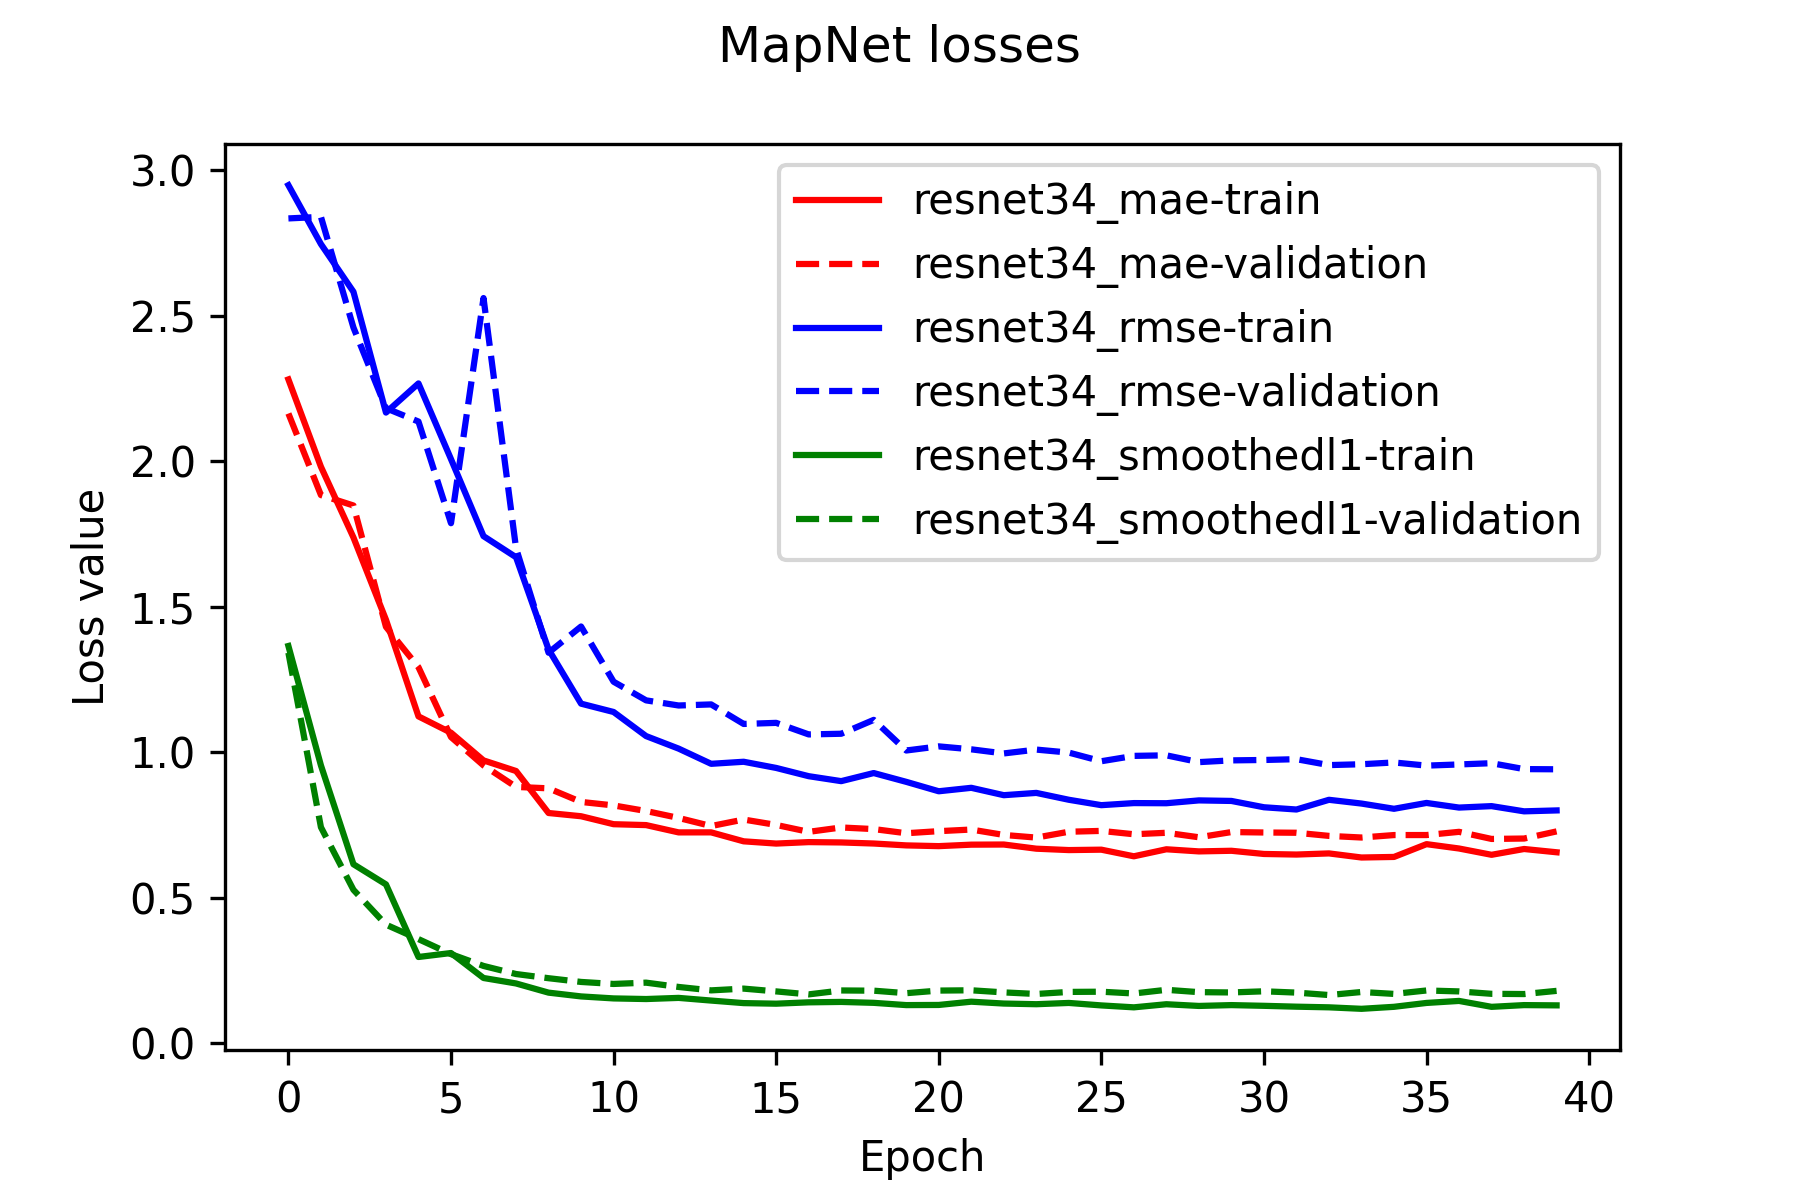
\includegraphics[width=0.50\textwidth]{./imgs/mapnet_losses.png}
    \end{center}
    \caption{MapNet (ResNet-34) losses}
    \label{fig:mapnet-losses}
\end{figure}

\begin{figure*}
    \begin{center}
        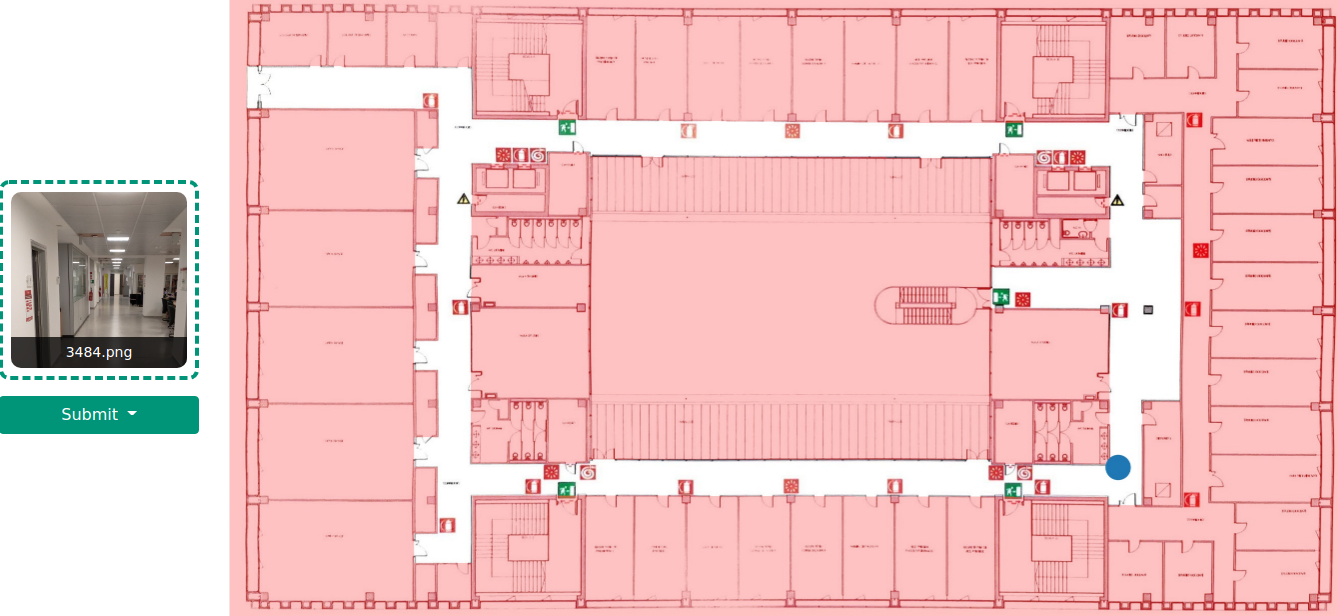
\includegraphics[width=0.95\textwidth]{./imgs/dashboard.png}
    \end{center}
    \caption{Inference dashboard}
    \label{fig:dashboard}
\end{figure*}


% accuracy with respect to different ResNets used. The bigger the ResNet, the better the results should be

% Some accuracies wrt. hyperparameters tuning

% Some plots on losses
